\section{Navigation}
\label{capter:high-level:navigation}

There is a plethora of specific phenomena for each of the five rubrics of interest that one might want to study.
Often, they align with a performance hypothesis such as ``the throughput per core might be low, as data never resides in the L3 cache''.
In this case, one would study the L3 cache access characteristics as phenomenon.
Running through different phenomena or hypotheses in an anarchic way following intuition is often not leading to the correct conclusion, as it runs risk that important details are missed out.
While the following sections---one for each of the five fundamental assessment dimensions---each host sets of effects to dive into, an overarching challenge is how these effects, aspects and things to study are properly structured.
For example, should we first study the bandwidth and then the latency behaviour before we look at vectorisation, or the other way round?

We originally intended to create something like a decision tree:
a unique, clear, deterministic guideline of which phenomena to study one after the other with the goal to come up with a clear explanation of why a code behaves the way it does.
Such a tree yielding a cascade of hypotheses to follow would provide a guideline that reads similar to:
First look at the load balancing.
If the load balancing is bad, fix it; otherwise have a look at the number of synchronisation points.
Then continue with false sharing.
And so forth. 
  
\begin{figure}[htb]
  \begin{center}
    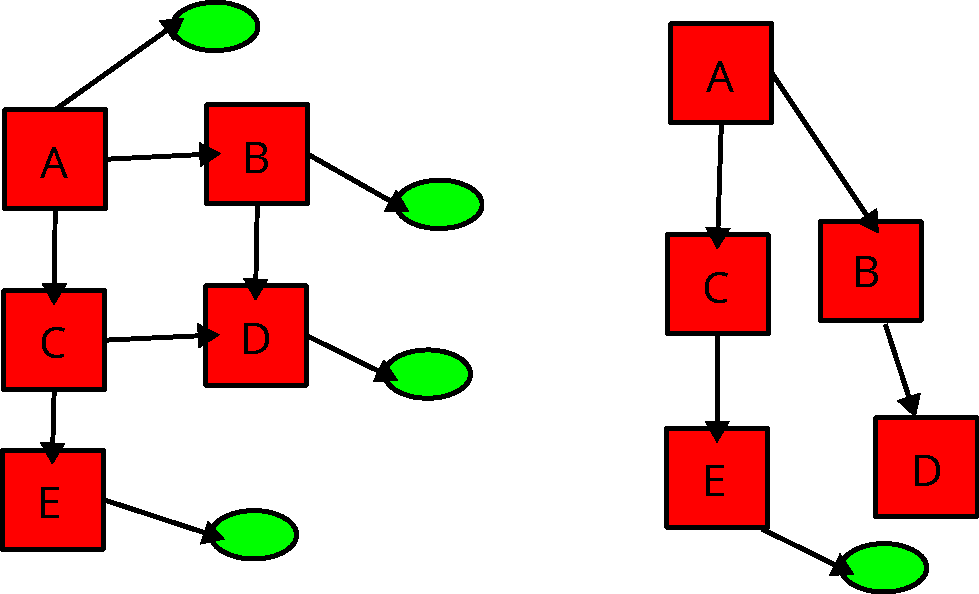
\includegraphics[width=0.6\textwidth]{workflow/graph-example.pdf}
  \end{center}
  \caption{
    Left: 
    In the example, we have a graph over hypotheses or effects (red squared) \texttt{A}--\texttt{E} that we might want to test for and that depend upon each other.
    Some hypothesis evaluations suggest certain explanations for the code's behaviour (green ellipses).
    In most cases, diving into one phenomenon will however require studying another follow-up hypothesis.
    As we work our way through the graph of hypotheses excluding more and more potential explanations,
    we build up a tree of hypotheses (right).
    This tree is analysis-specific, i.e.~might look different for the next case study.
    \label{figure:workflow:navigation}
  }
\end{figure}

Initial assessments with trial trees made it clear to us that such a decision tree is very difficult to construct.
Indeed, it is not clear whether a universally acceptable hypothesis tree to assess performance does exist. 
Different people have different ideas and preferences of what such a tree should look like, and these should be accommodated to keep motivation high and to allow people in the way that is most effective and constructive to them.
Further to that, it might be reasonable and valuable to use a tailored tree per assessment exercise and code:
every code is different, so the best-case sequence of effects to analysis is different, too. 

Therefore, we propose to arrange performance hypotheses to study in a directed graph (Figure~\ref{figure:workflow:navigation}).
It is the assessor's duty to navigate this graph to find explanations.
For each code assessment, the analysis journey might yield a different traversal of the graph.
Implicitly, each assessment will yield a decision tree informed by the graph:
We run through a sequence of hypotheses.
For each hypothesis, there might be multiple options where to go next, and the assessor picks one.
That might lead into a dead end, so we return to an earlier hypothesis that we didn't follow-up immediately.


It does not matter in which order we run through the graph of tests and hypotheses.
However, it matters that we stick to their systematic order and do not jump into an arbitrary node right from the start.
If we do this, we might miss out of context and alternatives; we work unscientifically.



\paragraph*{How it works}

\begin{itemize}[noitemsep]
  \item[$\boxplus$] Navigate through the graph of phenomena and hypotheses one by one.
  \item[$\boxplus$] Keep track of the effects analysed and record the resulting decision tree.
\end{itemize}


\paragraph*{How it does not work}

\begin{itemize}[noitemsep]
  \item[$\boxminus$] Aim for a decision tree that can universally and mechanically be applied to all benchmarks.
  \item[$\boxminus$] Pick different phenomena to look at randomly without following the causal dependencies encoded within the decision graph.
\end{itemize}
